\section{Introduction}

\begin{wrapfigure}{r}{.50\textwidth}
%(λx.λy. x) a b
%\begin{figure}
    \centering
    \begin{diagram}[width=0.45\textwidth]
import Diagrams.Prelude hiding (trace, _fontSize)

import NotionalMachines.Lang.UntypedLambda.Main (Exp (..), parse)
import NotionalMachines.LangInMachine.UntypedLambdaExpressionTree (diagramTrace)
import NotionalMachines.Machine.ExpressionTree.BubbleDiagram (toDiagram', _fontSize, _framePadding)
import NotionalMachines.Meta.Steppable (Steppable (trace))
import NotionalMachines.Util.Diagrams (diagramWithError)
import NotionalMachines.Examples.Diagrams (langAndNMTrace)

toDia = toDiagram' (def { _fontSize = 0.12, _framePadding = 0.04 })
t = langAndNMTrace 0.05
                   (diagramTrace toDia)
                   (fmap trace . parse)

dia = (diagramWithError . t)
      "(\\t. \\f. t) a b"
    \end{diagram}
    \caption{Evaluation of the term $\texttt{\app{\app{(\abs{t}{(\abs{f}{t})})}{a}}{b}}$ shown with the \nm{} \nmName{ExpTree}.}
    \label{fig:takeFirst}
%\end{figure}
\end{wrapfigure}

% - learning programming an notional machines
Learning to program involves learning how to express a program in a programming language, 
but also learning what the semantics of such a program is. 
For novices, the semantics of a program is often not obviously apparent from the program itself.
% - what is an NM?
Instructors then often use a \emph{\nm{}}~\citep{fincherNotionalMachinesComputing2020} to help teach
some particular aspect of programs and programming languages,
and also to assess students' understanding of said aspect.
%
This aspect is the \nm{}'s focus.
%
% - an example
For example, showing expressions as trees (the \nmName{ExpTree} \nm{}),
as depicted in Figure~\ref{fig:takeFirst},
brings out the internal structure of lambda-calculus expressions~\citep{marceauValuesGrowTrees2011}
and can help to explain the step-by-step evaluation of such expressions. 
%
% Note the two dimensions that play a role here:
% showing some aspect of a programming language (showing the expression as a tree), and
% performing an operation on it (a step in the evaluation of an expression). 
%A NM should help a novice in understanding the aspects for which the NM has been designed.
\Nms{} are used widely in computer science education;
\citet{fincherNotionalMachinesComputing2020} interviewed computer science teachers
to build up a dataset of \numOfNMs{} \nms{}%
\footnote{\url{https://notionalmachines.github.io/notional-machines.html} -
The website lists 57 items but some of them are part of what they call a \nm{} sequence,
which we consider a single \nm{}.}.


% - the quality of an NM is important.
\subsection{Unsound \NMs{}}
\label{sec:UnsoundNotionalMachines}

Given the extensive use of \nms{},
and
their intended use as devices to help students when learning,
it is important to look at their quality.
%Obviously, a \nm{} should be tested in practice
%%
%to answer questions such as
%``how well do students understand a particular aspect after studying it using a particular \nm{}?''
%and
%``what is the cost associated with introducing the notional machine
%(how much time had to be invested to obtain a benefit)?''.
%%
% But even before experimenting with a \nm{},
%%
% The first quality attribute we should be concerned with is to
To begin with,
one should
make sure that the \nm{} is \emph{sound}:
% correct
% consistent
% accurate
it is
%in some sense
faithful to the aspect of programs it is meant to focus on.
%
% Feynman quote
Anecdotal evidence of using unsound representations in education goes back a long way.
%
In 1960, education pioneer Jerome Bruner wrote that
``the task of teaching a subject to a child at any particular age is one of representing the structure of that subject in terms of the child’s way of viewing things'', that this
``task can be thought of as one of translation'', but that ideas have to be
``represented \emph{honestly} […] in the thought forms of children''~\cite{ brunerProcessEducation1960}.
Bruner’s use of the term ``honestly'' can be seen as a call for soundness of such representations.
%
Decades later,
Richard Feynman eloquently stated~\citep{feynmanSurelyYouRe1985},
after reviewing ``seventeen feet'' of new mathematics schoolbooks for the California State Curriculum Commission:

\begin{quote}
    %... the books were so lousy.
    %They were false. They were hurried.
    [The books] would try to be rigorous, but they would use examples
    (like automobiles in the street for ``sets'')
    which were almost OK, but in which there were always some subtleties.
    The definitions weren't accurate.
    Everything was a little bit ambiguous.
    %---they weren't smart enough to understand what was meant by ``rigor.''
    %They were faking it.
    %They were teaching something they didn’t understand, and
    %which was, in fact, useless, at that time, for the child.
\end{quote}

Ambiguously specified \nms{}
and
\nms{} with imperfect analogies to programming concepts
are a problem.
Educators may mischaracterize language features and
students may end up with misconceptions~\citep{chiodiniCuratedInventoryProgramming2021} instead of profoundly understanding the language.

% saves about 20 lines of text
\begin{wrapfigure}{r}{.50\textwidth}
% \begin{figure}[h]
    \centering
    \begin{tabular}{c}
        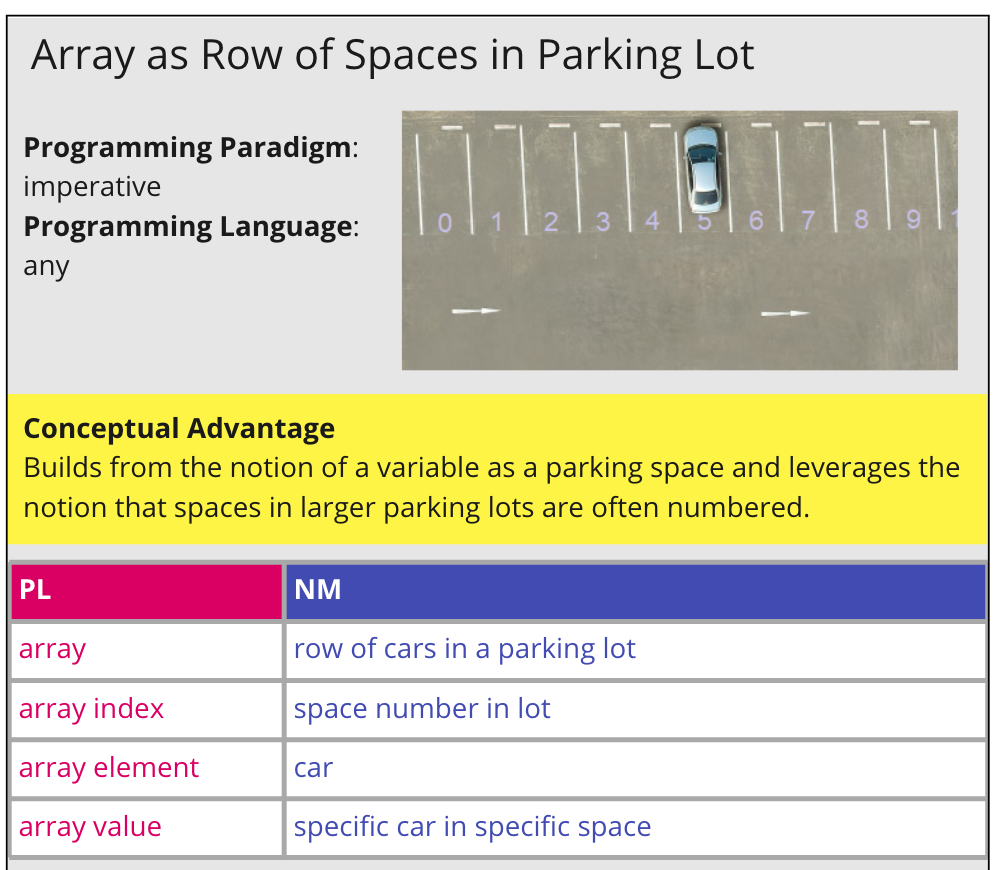
\includegraphics[width=.50\textwidth]{images/nm-definition-cards/nm-array-as-row-of-spaces-in-parking-lot-cut}
    \end{tabular}
     \caption{The ``Array as Row of Spaces in Parking Lot'' \nm{} captured by~\citet{fincherNotionalMachinesComputing2020}.}
    \label{fig:parkingSpaces}
% \end{figure}
\end{wrapfigure}

% - example: Array as Row of Parking Spaces
For example,
\citet{fincherNotionalMachinesComputing2020} describe the
``Array as Row of Spaces in Parking Lot'' \nm{}.
Figure~\ref{fig:parkingSpaces} shows part of their card summarizing it.
Notice the parallels between the programming language (PL) and the notional machine (NM).
% problem: empty parking space
Consider Java, a language commonly used in programming courses.
In Java,
when an array of objects is allocated,
all its slots contain
\mintinline{java}{null},
which means these slots don't contain a reference to any object.
This would be reasonably represented in the notional machine as an empty parking lot.
But if instead of an array of objects, we have an array of
\mintinline{java}{int}s,
for example,
then when we instantiate an array,
all its slots contain
\mintinline{java}{0},
which is not the absence of a number but a number like any other.
%
% other problems
A student could also reasonably question whether
one can park a car in a slot that is already occupied by another car,
or whether
one has to remove a car from a spot to park another car in the same spot.
%
In fact, the authors point out that,
``the effectiveness of the analogy depends on
%student knowledge of numbered parking spaces and
[...]
how well that models the semantics of the programming language.''


% - What properties should a NM satisfy?
\subsection{Soundness of \NMs{} via Simulation}
To avoid
these issues,
we need to make sure that a \nm{} 
is indeed an accurate abstraction.
%
Although
the more general view of
notional machines
as ``pedagogic devices to assist the understanding of some aspect of programs or programming''~\citep{fincherNotionalMachinesComputing2020}
makes no direct reference to programming languages,
programs are expressed in programming languages
% be it text based or not
so we will look at these ``aspects of programs''
through the lens of how they are realized by some programming language.
%
If a \nm{}
represents
a part of the operational semantics of a programming language,
for example,
then
this
representation
should be sound, in the sense that
steps in the \nm{}
correspond to steps in the operational semantics of the programming language.

%We say,
%informally,
%that
%a \nm{} is \emph{sound} if it is: 
%\begin{itemize}
%    \item a proper abstraction: it represents one or more aspects of the programming language and no superfluous aspects;
%    \item consistent with the corresponding programming language: steps in the \nm{} correspond to steps in the language semantics, and lead to similar results.
%\end{itemize}

Showing the soundness of a \nm{}
% with respect to some lang?
amounts to demonstrating that
the \nm{} \emph{simulates}
(in the sense described by~\citet{milnerAlgebraicDefinitionSimulation1971})
%the operational semantics of the underlying programming language
the aspect of programs under the focus of the \nm{}.
%This aspect under focus can be, for example, the operational semantics of a programming language.
% More precisely, the \nm{} simulates the operations of the semantics that it focuses on.
%
This property can be given in the form of a commutative diagram.
%We will present several such diagrams throughout this work.
%
Milner's simulation was also used
by~\citet{hoareProofCorrectnessData1972}
to establish a definition of
the correctness of
an `abstract' data type representation
with respect to
its corresponding `concrete' data type representation.
%
\citet{cousotAbstractInterpretationUnified1977} use a similar commutative diagram to simulate concrete computations in their abstract interpretation framework.
%
This interpretation of simulation
also captures the relationship between a \nm{} and the underlying programming language
because
% that's exactly what
a \nm{} is indeed an \emph{abstraction} of some aspect of interest.


\subsection{Contributions}
% - contributions
This paper makes the following contributions:
\begin{itemize}
    \item A formal definition of sound \nm{} based on simulation (Section~\ref{sec:soundnessDefinition}).
    \item A methodology for designing \nms{} that are sound by construction.

        It consists of
        deriving part of the notional machine
        by leveraging
        the relationship between
        the abstract representation of the notional machine
        and
        the abstract syntax of the programming language under its focus.

        We demonstrate the methodology by applying it
        to a combination of various
        small programming languages,
        \nms{},
        and
        aspects of programming language semantics
        (Section~\ref{chr:Modeling}).

    \item A methodology for analyzing \nms{} with respect to their soundness.

        It consists of
        modelling the notional machine and
        the aspect of the programming language under its focus,
        %
        relating them via simulation. %and
        %
        %using property-based testing to find counterexamples where the simulation fails.

        We
        demonstrate
        %evaluate
        the methodology by
        % applying it
        analyzing
        % \emph{M2} is applied to
        existing \nms{},
        sometimes
        pointing out unsoundnesses, and suggesting directions for improvement (Section~\ref{chr:RevealingInconsistencies}).
\end{itemize}

A brief discussion about the distinction between the abstract and concrete representations of a notional machine
follows
in Section~\ref{sec:ConcreteSyntax}.
We then
evaluate, in Section~\ref{chr:Evaluation}, the entire framework  %we are proposing to reason about notional machines
by comparing the notional machines that appeared
in Section~\ref{chr:Modeling} and Section~\ref{chr:RevealingInconsistencies}
to an existing dataset of \numOfNMs notional machines.
We classify the notional machines in the dataset according to various dimensions and show that the notional machines we analyzed are representative of the design space of notional machines used in practice.
Section~\ref{sec:RelatedWork} discusses related work
and Section~\ref{sec:Conclusions} concludes.



